
%(BEGIN_QUESTION)
% Copyright 2008, Tony R. Kuphaldt, released under the Creative Commons Attribution License (v 1.0)
% This means you may do almost anything with this work of mine, so long as you give me proper credit

In this time-delay relay circuit, the motor will immediately start when the pushbutton is pressed, and continue to run for about 5 seconds after the pushbutton is released.  The green light-emitting diode (LED) is supposed to be on whenever the motor is stopped, and off whenever the motor is running:

$$\includegraphics[width=15.5cm]{i03169x01.eps}$$

However, a problem has developed with this circuit.  The green LED always remains on and the motor never starts, no matter what is done with the pushbutton switch.  Based on this information, determine the following:

\vskip 10pt

\begin{itemize}
\item{} \underbar{Two} components or wires in the circuit that you know cannot be failed either open or shorted, besides the 24 volt source.
\vskip 40pt
\item{} \underbar{Two} components or wires in the circuit you think could possibly be bad (either one independently capable of causing the problem), and the type of failure each would be (either open or shorted).
\end{itemize}

\vfil 

\underbar{file i03169}
\eject
%(END_QUESTION)





%(BEGIN_ANSWER)

This is a graded question -- no answers or hints given!

%(END_ANSWER)





%(BEGIN_NOTES)

The fact that the motor never starts and the LED always remains on tells us the relay contacts are never being actuated.  Thus, we are looking for faults which could prevent the relay coil from energizing, rather than faults that might interrupt power to the relay contacts or power through the motor.

\vskip 10pt

\goodbreak
\noindent
{\bf Components known to be in good working condition:}

\begin{itemize}
\item{} Wire from TP1 to TP4
\item{} All wires from TP2 to LED cathode
\item{} $R_1$
\item{} LED
\end{itemize}

\vskip 10pt

\goodbreak
\noindent
{\bf Components which could possibly be faulted:}

\begin{itemize}
\item{} Relay coil failed open.
\item{} Pushbutton switch failed open.
\item{} Wire from TP3 to coil failed open.
\end{itemize}

%INDEX% Troubleshooting review: electric circuits

%(END_NOTES)


